% ============================================================
% Lecture 4 -- Introduction to Linear Models
% ============================================================
\section{Introduction to Linear Models}\label{sec:L04}

\lectureheader{4}{TPJmhTmm4h0}{Week-2 slides \texttt{Feb2.pdf} (recap and ``Model: Aims and Methods'', heights data), with the instructor's handwritten annotations}

\begin{guiding*}
By the end of this lecture you should be able to:
\begin{itemize}
  \item state the aim of modelling: to find a low-dimensional summary of the relationship between a response $y$ and an explanatory variable $x$;
  \item explain ``all models are wrong but some are useful'' with an example;
  \item describe the heights data and use a jittered scatter plot;
  \item explain the training / validation / test split used to judge models.
\end{itemize}
\end{guiding*}

\subsection{Recap}
Week~1 introduced the layered grammar of graphics: scatter plots, smooth lines, bar charts,
polar coordinates and faceting. The instructor calls it the key tool in data visualisation.
Week~2 turns from \emph{looking} at data to \emph{modelling} it. The slides warn that there is
no statistical analysis yet: this week introduces the linear model exploratorily, to see
\emph{how it works}. The formal theory starts in Week~3 (\cref{sec:L08}).

\begin{note}[Practical instruction from the slides]
Download the data sets and the Week-2 R code from the course web page and keep them in the same
directory, set as R's working directory. The Python notebooks follow the same idea. All data
sets are in the project's \texttt{data/} folder, and the notebooks find it by a relative path.
\end{note}

\subsection{Aims of modelling}
\begin{definition}[Response and explanatory variable]\label{def:L04-vars}
We observe pairs $\{(x_i,y_i):1\le i\le n\}$. The variable $x$ is the
\vocab{independent} (explanatory) variable and $y$ the \vocab{dependent} (response)
variable. A \vocab{model} is a low-dimensional summary of the data set that captures the
patterns in the data, and in particular the way $y$ depends on $x$. It can then be used for
\emph{prediction}: given a new $x$, what $y$ should we expect?
\end{definition}

\begin{note}[Caution: all models are wrong, but some are useful]
The slides quote G.\,E.\,P.~Box's aphorism. The instructor's example is the ideal gas law
$PV=RT$. No real gas satisfies it exactly, yet it is a good approximation, and it helps us
\emph{understand the system}. A linear model is judged the same way: not by being true, but by
being a good enough approximation to be useful.
\end{note}

In practice, the slides list the questions one asks:
\begin{itemize}
  \item What hypotheses do we want to test with the data?
  \item How do we judge which model works better? One common method is to split the data into three parts: about $60\%$ for \vocab{training} (fitting the models), $20\%$ for \vocab{query} or validation (choosing between models), and $20\%$ for \vocab{testing} (evaluating the chosen model's performance on data it has never seen).
\end{itemize}

\subsection{The heights data}
\begin{example}[Pearson's mothers and daughters]\label{ex:L04-heights}
Between 1893 and 1898, Karl Pearson (the slides write E.\,S.~Pearson) and his colleagues collected
the heights of mothers and their adult daughters in Britain. The version used in the course
(\texttt{heights.txt}; \texttt{Heights} in the R package \texttt{alr4}) has $n=1375$ pairs. The
annotations mention ``about 1500 odd'' and the restriction to daughters aged at least $18$
and mothers under $65$.
\begin{itemize}
  \item \texttt{Mheight}: height of the mother (inches), mean $62.45$;
  \item \texttt{Dheight}: height of one adult daughter (inches), mean $63.75$.
\end{itemize}
The \emph{object of study} is the question: \emph{how does the daughter's height depend on the
height of the mother?}
\end{example}

Heights were rounded to the nearest inch in the original records, so many points coincide. A
\vocab{jitter plot} moves each data point by a small uniformly distributed amount, here
$U(-0.5,0.5)$ in each coordinate, so that overlapping points become visible.

\begin{figure}[ht]
\centering
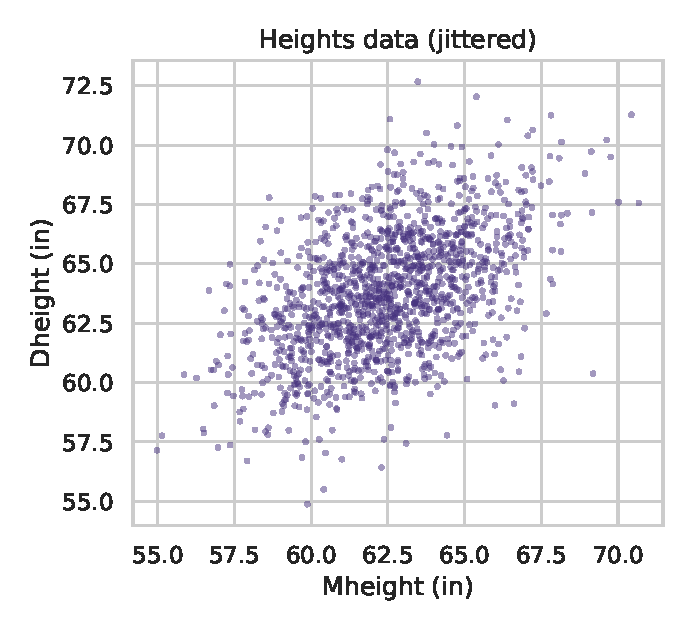
\includegraphics[width=0.5\textwidth]{figures/L04_heights.pdf}
\caption{Jittered scatter plot of daughter's height against mother's height.}
\label{fig:L04-heights}
\end{figure}

The instructor then restricts attention to the middle of the plot: mothers between about $58$
and $68$ inches. His annotations point out two features. There are \emph{no unusually tall
daughters of short mothers}, and \emph{no short daughters of very tall mothers}. The scatter
drifts upwards: taller mothers tend to have taller daughters. The plan is to develop a
technique that fits a linear model to the data $\{(x_i,y_i)\}$, that is, to find $a_1,a_2$ such
that
\[
y = a_1 + a_2 x
\]
is a good approximation. The technique is least squares. It is built step by step in
\cref{sec:L05}. It can also identify outliers: points far from the fitted line.

\begin{note}[Supplementary: the fitted line and ``regression to the mean'']
Anticipating \cref{sec:L05}, the least-squares line for these data is
\[
\widehat{\text{Dheight}} = 29.917 + 0.542\,\text{Mheight}, \qquad R^2 = 0.241.
\]
The slope $0.54<1$ means that a mother who is $1$ inch taller than average has a daughter who is
on average only about half an inch taller than average. This is Galton's \emph{regression to the
mean}. The word ``regression'' comes from this phenomenon. $R^2$ is defined in \cref{sec:L17}.
Only about a quarter of the variation in daughters' heights is explained by mothers' heights.
\end{note}

\begin{figure}[ht]
\centering
\begin{tikzpicture}[>=stealth]
\draw[->] (0,0) -- (7,0) node[right] {$x$};
\draw[->] (0,0) -- (0,4.2) node[above] {$y$};
\foreach \x/\y in {0.8/1.4,1.3/1.1,1.8/2.0,2.4/1.7,3.0/2.6,3.5/2.2,4.1/3.1,4.6/2.8,5.2/3.6,5.8/3.3,6.3/3.9}
  \fill (\x,\y) circle (1.5pt);
\draw[thick,red] (0.4,1.0) -- (6.6,3.9) node[right] {$y=a_1+a_2x$};
\draw[blue,dashed] (3.5,2.2) -- (3.5,2.38);
\draw[blue,dashed] (4.1,3.1) -- (4.1,2.66);
\node[blue,font=\small] at (4.9,1.4) {residual $=y_i-(a_1+a_2x_i)$};
\draw[blue,->] (4.5,1.6) -- (4.12,2.8);
\end{tikzpicture}
\caption{The goal: a line $y=a_1+a_2x$ that summarises the cloud of points. The vertical gaps
are the residuals studied in \cref{sec:L05,sec:L06}.}
\label{fig:L04-line}
\end{figure}

\subsection{Computation}
The R code reads \texttt{heights.txt} and plots \texttt{Dheight} against \texttt{Mheight}, with
jitter. In Python:
\codeline{h = pd.read\_csv(DATA / "Heights.csv"); plt.scatter(h.mheight + rng.uniform(-.5,.5,len(h)), h.dheight + rng.uniform(-.5,.5,len(h)))}
The notebook \nb{week02/L04\_intro\_linear\_models.ipynb} also demonstrates a 60/20/20 split.

\subsection{Summary}
\begin{itemize}
  \item A model is a low-dimensional summary of how the response $y$ depends on $x$. It is used for understanding and prediction.
  \item All models are wrong, but some are useful ($PV=RT$).
  \item Heights data: $1375$ mother--daughter pairs. Jittering reveals overlapping points. Taller mothers tend to have taller daughters.
  \item Goal: find $a_1,a_2$ so that $y\approx a_1+a_2x$. Models are compared using training/validation/test splits.
\end{itemize}

\subsection{Exercises}
\begin{problem}\label{prob:L04-1}
Why does jittering by $U(-0.5,0.5)$ not change any conclusion drawn from the plot, while it would change a fitted line if we fitted to the jittered data? By how much can the mean of the jittered $x$'s differ from the true mean in expectation?
\end{problem}
\begin{problem}\label{prob:L04-2}
Split the heights data at random into $60/20/20$ parts (with a fixed seed). Fit the line to the training part and compute the mean squared prediction error on the test part.
\end{problem}
\begin{problem}\label{prob:L04-3}
Give another physical law (like $PV=RT$) that is ``wrong but useful'', and say in what regime it fails.
\end{problem}
\begin{problem}\label{prob:L04-4}
Suppose daughters' heights were \emph{exactly} equal to their mothers'. What would the scatter plot look like, and what would $a_1,a_2$ be?
\end{problem}

\subsection{Further reading}
Weisberg, \emph{Applied Linear Regression} (4th ed.), Chapter~1 (Scatterplots and Regression),
which is the source of the heights, Forbes, bass and snowfall examples. Wickham \& Grolemund,
\emph{R for Data Science}, ``Model basics''. Christensen, Chapter~6 (Regression analysis) for
the formal treatment.
